% +--------------------------------------------------------------------+
% | Appendix A Page (Optional)                                         |
% +--------------------------------------------------------------------+

\cleardoublepage

\chapter{Guía de instalación para el servidor}
\label{Appendix:Key1}

\section{Docker}
\label{makereference7.1}
Esta es una guía para el despliegue del servidor en Docker.

Para ello primero tenemos que tener una instancia de docker, si se quiere ejecutar en local, 
hay que instalar docker por el enlace \url{https://www.docker.com/}
La imagen de docker se descarga por git por el siguiente enlace:
\url{https://github.com/ZReKoJ/Docker.git}

\begin{lstlisting}[language=bash, caption=Dockerfile]
    FROM ubuntu:16.04

    RUN apt-get update 
    RUN apt-get install -y openssh-server
    RUN mkdir /var/run/sshd
    RUN echo 'root:tfg-ucm' | chpasswd
    RUN sed -i 's/PermitRootLogin prohibit-password/PermitRootLogin
         yes/' /etc/ssh/sshd_config
    
    # SSH login fix. Otherwise user is kicked off after login
    RUN sed 's@session\s*required\s*pam_loginuid.so@session optional
         pam_loginuid.so@g' -i /etc/pam.d/sshd
    
    ENV NOTVISIBLE "in users profile"
    RUN echo "export VISIBLE=now" >> /etc/profile
    
    EXPOSE 22 8000 8080
    CMD ["/usr/sbin/sshd", "-D"]
\end{lstlisting}

\begin{lstlisting}[language=bash, caption=Descarga de la imagen de docker]
    # Descarga de la imagen
    git clone https://github.com/ZReKoJ/Docker.git 
    # Entrar en la carpeta
    cd Docker 
    # Crear la imagen
    docker build --tag=filmar . 
\end{lstlisting}

\begin{figure}[H]
    \centering
    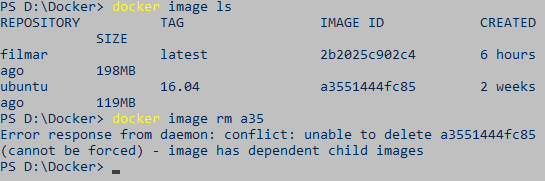
\includegraphics[width=6in]{figures/appendix-A/list-docker-images.png}
    \caption{Imágenes creadas de docker}
\end{figure}

Se han creado dos imágenes tras la ejecución, la de ubuntu es una dependencia usada, para tener el entorno de linux, por eso no se puede borrar.

\begin{lstlisting}[language=bash, caption=Levantamiento de la instancia de docker]
    # Levanta docker mapeando puertos
    docker run -p 22022:22 -p 8080:8080 filmar 
    # No hace falta ejecutar los siguientes comandos
    # Comando para listar containers de docker corriendo
    docker ps 
    # Listar todos los containers
    docker container ls --all 
    # Parar el container
    docker stop 018 
    # Borrar el container
    docker rm 018 
\end{lstlisting}

\begin{figure}[H]
    \centering
    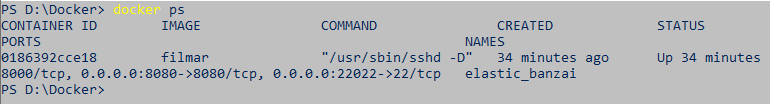
\includegraphics[width=6in]{figures/appendix-A/list-docker-containers.png}
    \caption{La instancia de docker levantada}
\end{figure}

Ahora que se ha levantado la instancia de docker con un ID 0186392cce18 y sus respectivos puertos mapeados.
Se conecta al container mediante ssh con la contraseña \textbf{tfg-ucm}

\begin{lstlisting}[language=bash, caption=Conexión ssh]
    # El puerto 22022 es el que se habia mapeado
    ssh root@localhost -p 22022
\end{lstlisting}

Una vez conectado al container, hay que instalar las siguientes herramientas

\begin{lstlisting}[language=bash, caption=Instalaciones]
    # Actualizacion por si acaso
    apt update 
    # Para descargar el repositorio en github
    apt install git
    # El servidor es un proyecto maven
    apt install maven
    # Base de datos
    apt install postgresql
    # Para usuarios
    apt install sudo
    # El servidor es un proyecto de java
    apt install openjdk-8-jdk
\end{lstlisting}

Una vez instalado todas las herramientas, descargar el proyecto del servidor,
que esta en \url{https://github.com/DanielCalle/TFG-Server.git}

\begin{lstlisting}[language=bash, caption=Descarga del proyecto]
    # Se recomienda descargar el proyecto en la carpeta home
    cd /home
    git clone https://github.com/DanielCalle/TFG-Server.git
\end{lstlisting}

Antes de levantar el servicio, hay que preparar postgresql. El archivo sql está dentro del proyecto
en el siguiente path: \url{/src/main/webapp/WEB-INF/sql/filmar_low.sql}

\begin{lstlisting}[language=bash, caption=Configuración postgresql]
    # Cambiar al usuario postgres (por defecto)
    sudo -i -u postgres
    # Iniciar psql
    psql
    # Cambiar el password a 'admin'
    \password
    # Creacion de una base de datos
    create database films;
    # Salir de psql
    \q
    # Crear la estructura de base de datos
    # Anadir datos
    psql -d films -f /home/TFG-Server/src/main/webapp/
        WEB-INF/sql/filmar_low.sql
    # Salir del usuario postgres
    exit
\end{lstlisting}

Una vez configurado postgres, se procede al despliegue del servicio.

\begin{lstlisting}[language=bash, caption=Despliegue]
    # Acceder a la raiz del repositorio
    cd /home/TFG-Server
    # Empaquetar con el perfil de docker
    mvn package -P Docker
    # Dar permiso de ejecucion al script
    chmod +x server.sh
    # Ejecutar 
    ./server.sh start
    # No hace falta ejecutar los siguientes comandos
    # Para parar el servicio
    ./server.sh start
    # Para reiniciar el servicio
    ./server.sh restart
\end{lstlisting}

Ya está levantado el servicio en el puerto 8080, se puede probar con el siguiente enlace
\url{localhost:8080/films}.

% +--------------------------------------------------------------------+
% | Enter text for your Appendix page in the space below this box.     |
% |                                                                    |
% +--------------------------------------------------------------------+
